%% ----------------------------------------------------------------
%% Background.tex
%% ----------------------------------------------------------------
\chapter{Background and report of literature search}

There were lots of different algorithms existing for object detection and tracking. Some of those algorithms were investigated in this project in order to identify a set of suitable algorithms that were both accurate and efficient enough to analysis video stream from camera in real-time.

\section{Background subtraction}

Being able to detect objects in a video frame is the first, also the most difficult and important step to do object tracking. This is generally accomplished by separation of foreground objects and background image. Three different object detection methodologies were investigated in this project.

\subsection{Colour based}

Colour can provides enough information of a specific object. For easier analysis of colour information, a hue-saturation-value (HSV) colourspace \cite[p.~301]{colourspace} representation converted from the original RGB colourspace is usually used, because it would be easier to filter a range of colour based on hue, saturation and brightness.

A simple colour based foreground mask can be generated easily by filtering target colour. An simple implementation \cite{MOTBOC.git} of colour filtering object detection algorithm was investigated, as shown in \fref{Figure:MOTBOC}.

\begin{figure}[H]
  \centering
  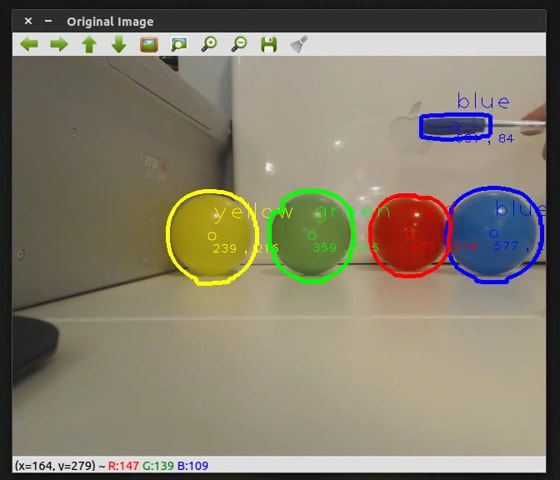
\includegraphics[width=0.6\columnwidth]{MOTBOC}
  \caption{Multi Object Tracking Based on Color (adapted from \cite{MOTBOC.git})}
  \label{Figure:MOTBOC}
\end{figure}

This implementation doesn't require a lot of computation, thus was very fast, could be suitable for robots that are tracking sonething like a single coloured ball or piece of paper, also could be useful for line racing car projects.

However, this implementation is very limited, it can only detects objects with single colour, cannot distinguishes the objects from similar background colour, relies heavily on manually adjusted colour threshold values, and is very sensitive to the variations of colourspaces from different cameras, not very adaptable. A complex environment may also results into lots of undesired detections, as shown in \fref{Figure:MOTBOC_F}.

\begin{figure}[H]
  \centering
  \includegraphics[width=0.6\columnwidth]{"MOTBOC failure"}
  \caption{Simple Multi Object Tracking Based on Color \cite{MOTBOC.git} at a complex environment}
  \label{Figure:MOTBOC_F}
\end{figure}

\subsection{Shape based}

Another important information about an object is its shape. By extracting hard object edges in the scene than apply appropriate shape transformation and filtering algorithms, an object could also be detected based on the shape.

\fref{Figure:circles} shows the image processed by circle detection, based on OpenCV's implementation of Hough Circle Transform \cite{opencv:hough_circle}. The coin at the top right corner had not been detected, because it actually appears to be a eclipse to the algorithm because of visual perspective.

\begin{figure}[H]
  \centering
  \subfigure [] {
    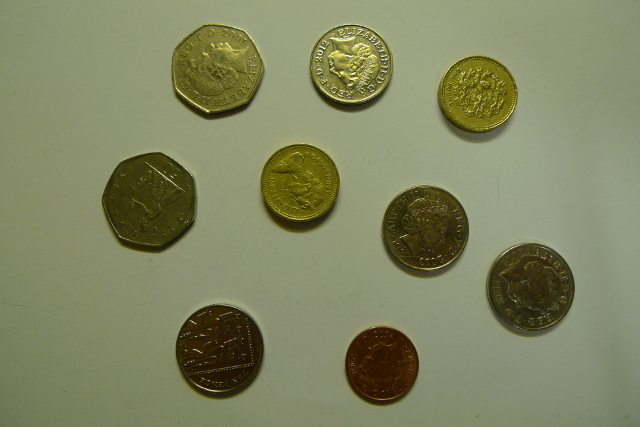
\includegraphics[width=0.45\columnwidth]{simple_original}
    \label{Figure:edges:original}
  }
  \subfigure [] {
    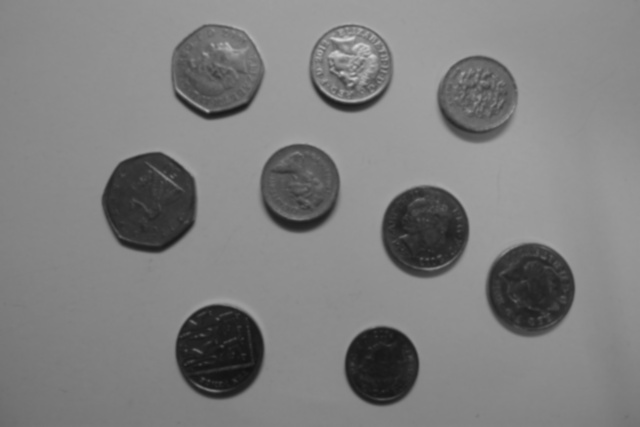
\includegraphics[width=0.45\columnwidth]{simple_blur}
    \label{Figure:edges:blur}
  }
  \subfigure [] {
    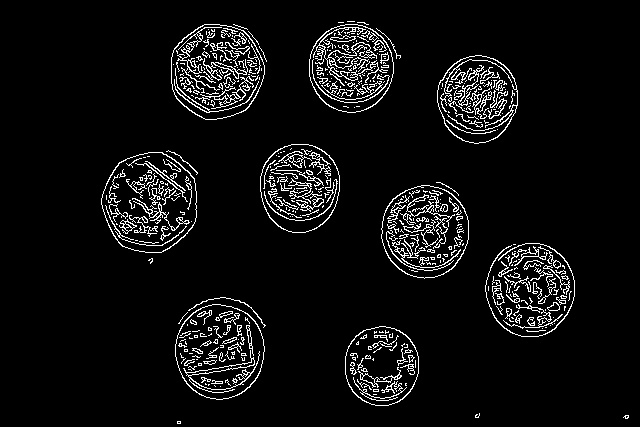
\includegraphics[width=0.45\columnwidth]{simple_edges}
    \label{Figure:edges:edges}
  }
  \subfigure [] {
    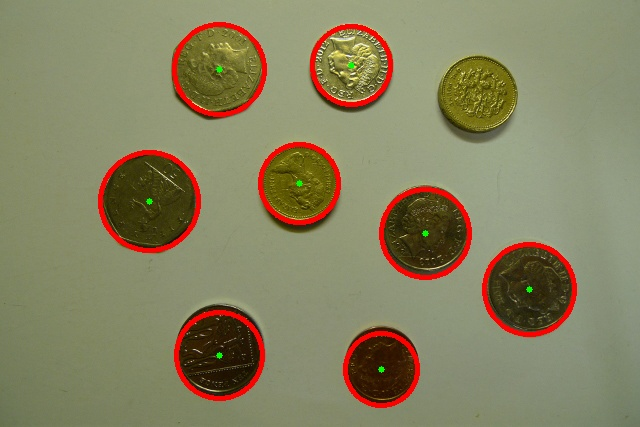
\includegraphics[width=0.45\columnwidth]{simple_circles}
    \label{Figure:edges:circles}
  }
  \caption{Circle detection. \subref{Figure:edges:original} The original image, \subref{Figure:edges:blur} image converted to gray scale and blurred, \subref{Figure:edges:edges} edges detected, \subref{Figure:edges:circles} circles detected}
  \label{Figure:circles}
\end{figure}

\subsection{Cascade Classifier}

Cascade classifier \cite{cascade} is another widely used technique for object detection. It concatenates several classifiers detecting different object features to recognise objects, and it can be trained both positively and negatively to improve accuracy. It was usually used for object classify, for example recognise human and different classes of vehicles in a single frame.

The OpenCV's cascade classifier implementation \cite{opencv:cc} of face and eye detection was investigated as shown in \fref{Figure:cc_face}.

\begin{figure}[H]
  \centering
  \includegraphics[width=0.6\columnwidth]{"CC face"}
  \caption{Face and eye detection cascade classifiers, detected face was circled by pink, whereas detected eyes were circled by blue}
  \label{Figure:cc_face}
\end{figure}

Noticeable frame rate drop and latency was experienced when using the cascade classifier implementation on the testing platform, suggests it was not a fast enough algorithm for real-time object tracking application. In addition, multiple classifier definition files were required for detecting different kinds of objects, or even different perspectives of the same object, which would require lots of computations.

\subsection{Motion based}

By differenceing current frame and previous frames, it is also possible to detects moving objects efficiently. The BGSLibrary \cite{bgslibrary} is specifically developed for this purpose, it offers 37 different background substraction algorithms using OpenCV, published under GNU GPL v3 license.

The article \cite{bgs:article} reviewed the algorithms available in the BGSLibrary, ranked 5 algorithms as the best methods for accuracy. Except the Pixel-Based Adaptive Segmenter (PBAS) algorithm which was removed due to patent issues, the other 4 algorithms listed in \tref{Table:bgs} were investigated in this project.

\begin{table}[H]
  \centering
  \begin{tabular}{cc}
  \toprule
  \textbf{Method ID} & \textbf{Method name}\\
  \midrule
  MultiLayerBGS & Multi-Layer BGS \\
  MixtureOfGaussianV1BGS & Gaussian Mixture Model \\
  LBAdaptiveSOM & Adaptive SOM \\
  DPWrenGABGS & Gaussian Average \\
  \bottomrule
  \end{tabular}
  \caption{Background substraction algorithms investigated (adapted from \cite{bgslibrary})}
  \label{Table:bgs}
\end{table}

\fref{Figure:bgs_frame} shows the foreground masks obtained from those 4 algorithms through 2 sample frame sequences available with the BGSLibrary \cite{bgslibrary}.

\begin{figure}[H]
  \centering
  \includegraphics[width=0.24\columnwidth]{bgs_frame/MultiLayerBGS/input}
  \includegraphics[width=0.24\columnwidth]{bgs_frame/MultiLayerBGS/mask}
  %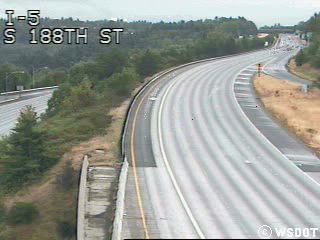
\includegraphics[width=0.32\columnwidth]{bgs_frame/MultiLayerBGS/bkgmodel}
  \includegraphics[width=0.24\columnwidth]{bgs_video/MultiLayerBGS/input}
  \includegraphics[width=0.24\columnwidth]{bgs_video/MultiLayerBGS/mask}

  \includegraphics[width=0.24\columnwidth]{bgs_frame/MixtureOfGaussianV1BGS/input}
  \includegraphics[width=0.24\columnwidth]{bgs_frame/MixtureOfGaussianV1BGS/mask}
  \includegraphics[width=0.24\columnwidth]{bgs_video/MixtureOfGaussianV1BGS/input}
  \includegraphics[width=0.24\columnwidth]{bgs_video/MixtureOfGaussianV1BGS/mask}
  %
\includegraphics[width=0.32\columnwidth]{na}

  \includegraphics[width=0.24\columnwidth]{bgs_frame/LBAdaptiveSOM/input}
  \includegraphics[width=0.24\columnwidth]{bgs_frame/LBAdaptiveSOM/mask}
  \includegraphics[width=0.24\columnwidth]{bgs_video/LBAdaptiveSOM/input}
  \includegraphics[width=0.24\columnwidth]{bgs_video/LBAdaptiveSOM/mask}
  %
\includegraphics[width=0.32\columnwidth]{na}

  \includegraphics[width=0.24\columnwidth]{bgs_frame/DPWrenGABGS/input}
  \includegraphics[width=0.24\columnwidth]{bgs_frame/DPWrenGABGS/mask}
  \includegraphics[width=0.24\columnwidth]{bgs_video/DPWrenGABGS/input}
  \includegraphics[width=0.24\columnwidth]{bgs_video/DPWrenGABGS/mask}
  %
\includegraphics[width=0.32\columnwidth]{na}
  \caption{Results obtained from background substraction algorithms. From left to right column: input sample 1, foreground mask obtained, input sample 2, foreground mask obtained. From top to bottom row: MultiLayerBGS, MixtureOfGaussianV1BGS, LBAdaptiveSOM and DPWrenGABGS.}
  \label{Figure:bgs_frame}
\end{figure}

It can be seen from \fref{Figure:bgs_frame} that MultiLayerBGS gave the best foreground masks, but it was also the slowest algorithm on the testing platform.

\section{Movement tracking}

After obtained the foreground object mask, they need to be interpreted as objects, then the object can be detected and tracked based on its position.

\subsection{Connected component analysis} \label{blob}

Connected component analysis, or Connected component labeling, is used for detecting connected regions (blobs). A blob detector can be used to mark and labeling individual objects from the foreground mask, therefore obtain parameters such as size, position and orientation of the object. Afterwards, by comparing nearby objects from previous frames, the objects can be tracked, and movement parameter such as velocity and acceleration can then be obtained by physical modelling.

There were also lots of free and open source blob detection libraries available, e.g. the simple blob detector came with OpenCV \cite{opencv:blob}, cvBlob library \cite{cvblob}.

This was not yet implemented at the time this progress report was written.

\subsection{Continuously Adaptive Meanshift}

Continuously Adaptive Meanshift (CAMshift) \cite{bradski1998computer} is a technique used to track a region of interest (ROI) in continuous frame sequences. It is based on Meanshift algorithm, which only track a fixed size ROI window, whereas CAMshift can handle target resize and rotation. In order to determine the ROI for CAMshift, the blob detector as described in Section \ref{blob} can also be used. This algorithm can also be easily implemented using OpenCV \cite{opencv:camshift}, and was used by lots of researches such as \cite{chu2007object}, \cite{xu2012moving} and \cite{nouar2006improved}.

This was not yet implemented at the time this progress report was written.
